% !TEX encoding = UTF-8 Unicode

% Beispiel für ein LaTeX-Dokument im Format "seminarvorlage"
\documentclass[ngerman]{seminarvorlage}
% ngerman = Deutsch in neuer Rechtschreibung, alternativ english
\usepackage[utf8]{inputenc} % Kodierung der Umlaute
\usepackage{babel} % automatische Sprachanpassung, Sprache siehe oben
\usepackage{cleveref} % für bequeme Referenzen, siehe \cref unten

%Own Code
\newcommand*{\fullref}[1]{\hyperref[{#1}]{\autoref*{#1} \nameref*{#1}}} % One single link
\newcommand*{\quelle}{% 
  \footnotesize Quelle: 
} 

\begin{document}

% Unbedingt angeben: Titel, Autoren, E-Mail
% Freiwillig: Adresse
\title{Embedded Realtime OS FreeRTOS auf STM32F4}
\numberofauthors{2}
\author{
  \alignauthor Michael Ebert\\
		\affaddr{Ad-hoc Networks GmbH}\\
    \email{ebert@ad-hoc.network}
  \alignauthor Christoph Bläßer\\
		\affaddr{Bundesamt für Sicherheit in der Informationstechnik}
    \email{christoph.blaesser@gmx.de}
}

\maketitle
\keywords{RTOS, ARM , STM32, Real Time.}

\abstract{
Im Rahmen des vorliegenden Papers wird das Echtzeitbetriebssystem FreeRtos vorgestellt. Hierzu werden zu Beginn die allgemeinen Vorgaben für Echtzeitbetriebssysteme beschrieben. Im Verlauf des Textes wird an ausgewählten Beispielen dargestellt, wie FreeRos diese Anforderungen berücksichtigt und durch geeignete Programmfunktionen umsetzt.
}
\section{Grundlagen}
\subsection{Allgemeine Anforderungen an Betriebssysteme}
Betriebssysteme verwalten den Hardwarezugriff und stellen sicher, dass eingesetzte Software die benötigte Rechenzeit zur Verfügung gestellt bekommt. Gleichzeitig regeln Sie den Hardwarezugriff und organiseren den konkurierenden Zugriff, beispielsweise auf Netzwerkkarten und Festplatten. Sie stellen Funktionen für die Interprozesskommunikation bereit udn übernehmen grundlegende Aufgaben wie die Organisation von Arbeitsspeicher.
\subsection{Echtzeitsysteme}
Mit der steigenden Leistungsfähigkeit von modernen $\mu$ Prozessoren, steigen auch die Anforderungen an die Software die auf diese Systeme aufsetzt. Viele dieser Systeme verlangen trotz ihrer Komplexität, dass Teile des Programmablauf in bestimmten zeitlichen Grenzen ausgeführt wird und somit vorhersehbar und deterministisch sind. Systeme die eine solche Anforderung unterliegen werden Echtzeitsysteme genannt. Echtzeitsysteme unterliegen einer weiteren Unterteilung in weiche und harte Echtzeitsysteme (soft / hard realtime systems). Ein weiches Echtzeitsysteme soll eine Aufgabe in den vorgegeben zeitlichen Grenzen ausführen, ein überschreiten ist aber erlaubt und führt nicht unmittelbar zu einem Fehler. Ein hartes Echtzeitsystem hingegen muss die gestellte Aufgabe in den vorgegebenen Grenzen ausführen. Eine Überschreitung macht das System unbrauchbar. Der Programmablauf eingebetteter Systeme lässt sich auf drei Grundmodelle zurückführen, siehe Abbildung \ref{fig:Programmablauf}. Eingebettete Anwendungen können in einer einzigen Schleife (mit und ohne Interrupt Unterbrechungen) laufen oder aber in event-gesteuerten nebenläufigen eigenständigen Programmabschnitten (Thread oder Task) ausgeführt werden. Diese Nebenläufigkeit ist nur durch einen RTOS Kernel (Scheduler) möglich. Ein RTOS Kernel abstrahiert Timing Informationen und kümmert sich darum, dass die nächste Task rechtzeitig ausgeführt wird. Der Entwickler ist dafür verantwortlich, dass die Task die gewünschte Aufgabe im zeitlichen Rahmen ausführt. Wie sichergestellt werden kann, dass Task  harten bzw. weichen Echtzeitanforderungen entspricht wird Abschnitt \ref{sec:Echtzeitanalyse} beschrieben. Für viele kleine Anwendungen kann die Nutzung einer einzigen Schleife durchaus sinnvoll sein, sollten beispielsweise die Ressourcen so knapp sein, dass ein Overhead an Funktionalität ausgeschlossen werden muss. Ein großer Nachteil der "`einschleifen Variante"' ist die permanente Nutzung des Prozessors. Besonders bei akkubetriebenen Geräten wie IoT Device oder Mobiltelefonen wird sehr genau auf die Energieaufnahme geachtet. Ein RTOS bietet hingegen Funktionen mit denen sehr leicht ermittelt werden kann, ob ein Gerät in einen Schlafmodus wechseln kann, dies wird in Abschnitt \ref{sec:Low Power Modes} an Beispielen von FreeRtos und einem ARM $\mu$Prozessor demonstriert. Neben der Echtzeitfähig gibt es aber noch viele weitere Vorzüge für den Einsatz eines Echtzeitbetriebssystems.  
Durch das Herunterbrechen der Anwendung in Task entstehen viele kleine Module, die jeweils eine kleine Teilaufgabe des Gesamtsystems übernehmen. Die Anwendungen werden so skalierbar und erweiterbar. Die Entwicklungsarbeit lässt sich leicht auf Teams verteilen, die unabhängig ihre Module (Tasks) entwickeln und testen. Dies ermöglicht auch den Einsatz von agilen Entwicklungsmethoden wie Scrum in der Entwicklung von eingebetteten Systemen. 
\newline
TODO Überleitung FreeRtos
\newline  
\begin{figure}
	\centering
		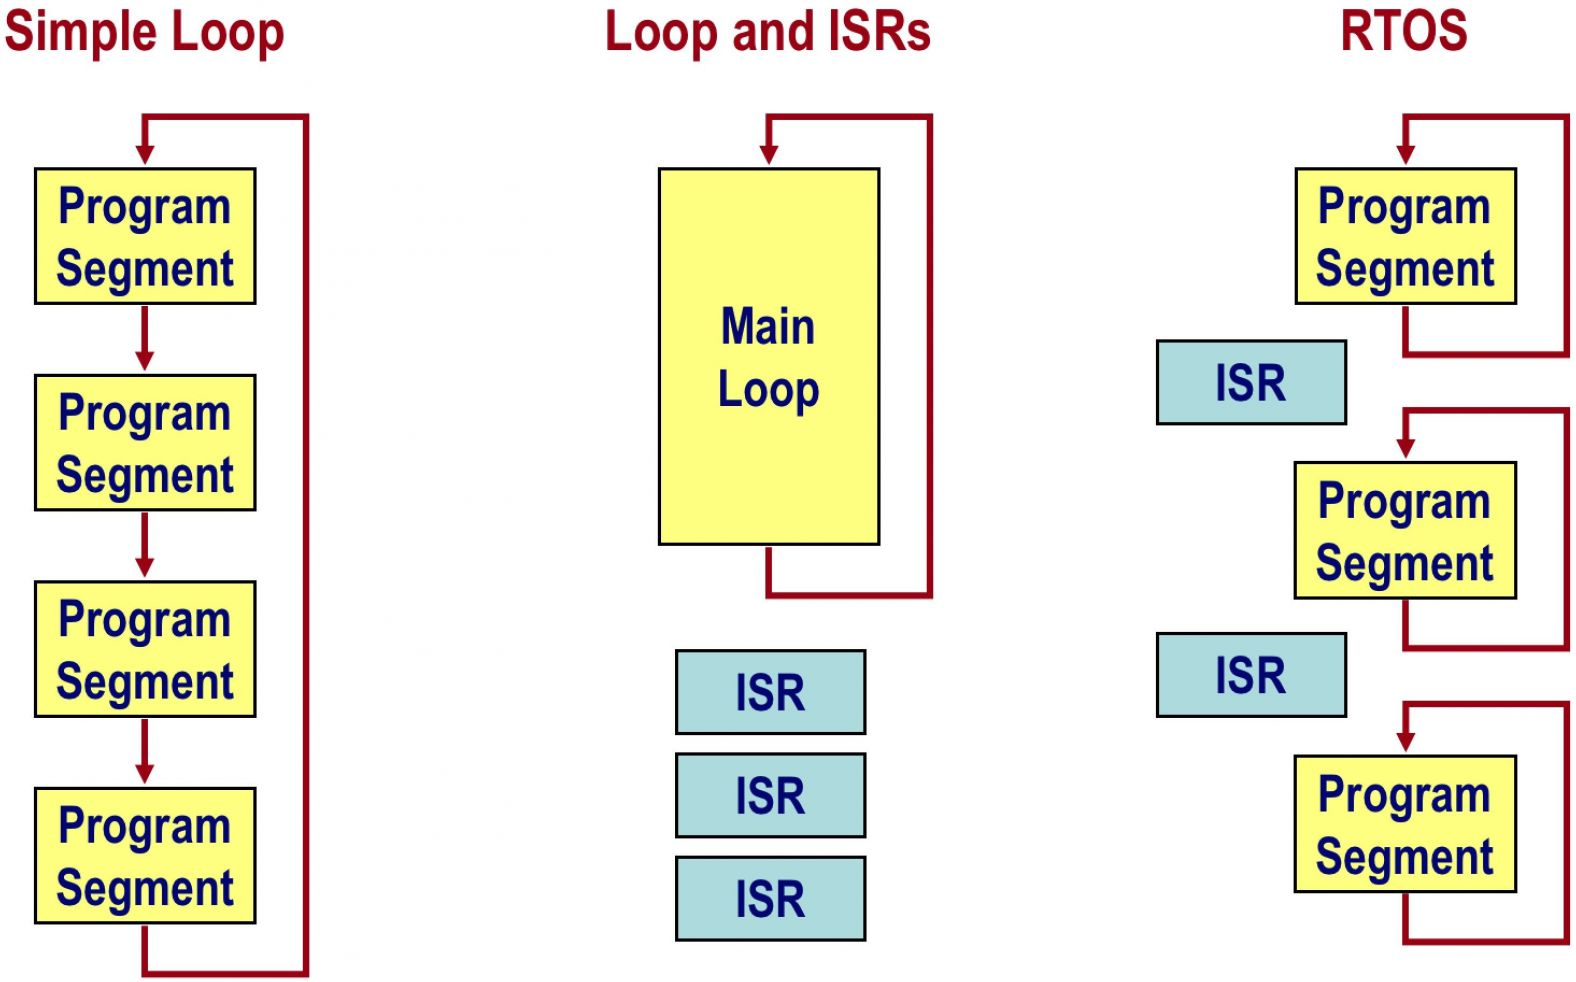
\includegraphics[width=0.3\textwidth]{Pictures/EmbeddedCom/cwrtos2f5c.jpg}
	\caption{Übersicht Programmabläufe}
	\quelle\url{http://www.embedded.com/}
	\label{fig:Programmablauf}
\end{figure}



\subsection{Anforderungen an Echtzeitbetriebssysteme}
Echtzeitbetriebssysteme kommen zum Einsatz wenn neben den oben genannten Anforderungen an ein normales Betriebssystem weitere Anforderungen gestellt werden, die ein normales Betriebssystem nicht berücksichtigt. Dies können beispielsweise garantiert berechenbare Reaktionszeiten sein wie sie in der Fabrikation oder im Automobilbereich gefordert werden oder geringe Leistungsaufnahmen wie bei Komponenten des Internet of Things (IoT). Insgesamt wird zwischen Harten und Weichen Echtzeitkriterien unterschieden. Diese Gliedern sich wie folgt:\newline
%%Zitat Anfang
\begin{itemize}
	\item Antwortzeiten
	\item Start-zu-Start Jitter von Tasks und Software-Komponenten
	\item Mehrfachaktivierung von Tasks
	\item Ausführungsreihenfolge von Software-Komponenten
	\item Latenzen von Wirkketten (Event Chains)
	\item Verlust von Daten
	\item Alter der Daten
	\item Datenkonsistenz
	\item Wiederverwendung von Daten
	\item Verlust von Interrupts
	\item Blockierung von Interrupts
\end{itemize}
%%Zitat Ende Quelle: http://www.inchron.com/fileadmin/INCHRON/3-PDFs/EN/Paper_IAV_Tagung_Sim_u_Test_B_Mai10_pdf.pdf


Aufgrund der Eingangs geschilderten Einsatzbereiche ist leich zu erkennen, dass Echzeitbetriebssysteme häufigin Umgebungen zum Einsatz kommen, in denen besondere Anforderungen an die Hardware gestellt werden. Häufig verfügt die Hardware nur über begrenzte Speicherkapazitäten, über geringe Wärmeableitfähigkeiten und damit geringe Rechenleistung. Die zur Verfügung stehende Energie muss bei der Entwicklung ebenfalls berücksichtigt werden. 
Vor diesem Hintergrund benötigen Echtzeitbetriebssysteme nur wenig Speicherplatz und implementieren Funktionen um den Prozessor und die angeschlossene Peripherie nur kurzzeitig zu belasten und in der restlichen Zeit in den Ruhezustand zu verseten.

\section{FreeRtos} 
\subsection{Geschichte}
\subsection{Zielsysteme}
\subsection{Entwicklungsumgebung}

\subsection{Fokus bei der Entwicklung}
\subsection{Ordner und Dateistrukturen} 
\subsection{Installation}
%nicht unbedingt eine Detailierte Beschreibung, jedoch genug Information, damit ein Dritter die Umgebung nachbauen und die Ergebnisse verifizieren kann.
\subsection{Scheduling}
\subsection{Memory Management}
\subsection{Interprozess Kommunikation}
\subsection{Software Timer}
\subsection{Interrupt Handling}
\subsection{Sonstige Maßnahmen zur Sicherstellung der Echtzeitfunktionalität}

\section{Entwicklungsumgebung}
\subsection{Eingesetzte Komponenten}
\subsection{Low Power Modes auf STM32F4 (ARM Cortex M3)}
\label{sec:Low Power Modes} 
%Hier nur, wenn es Teil der Umgebung ist, sonst weiter nach hinten.


\section{Echtzeitanalyse}
\label{sec:Echtzeitanalyse} 
\section{Debugging von Echtzeitsystemen} 
\section{Echzeit Pattern} 
\section{Komplexität durch Nebenläufigkeit} 
\section{Zusammenfassung}
\pagebreak
\bibliographystyle{abbrv}
\bibliography{literatur} % Daten aus der Datei literatur.bib verwenden.

\end{document}

